\documentclass[11pt, reqno]{article}

\usepackage{amsmath, amsthm, amssymb}
\usepackage{enumitem}
\usepackage{tcolorbox}
\usepackage{hyperref}
\usepackage{tikz}
\usepackage{tikz-cd}
\usepackage{pgfplots}
\pgfplotsset{compat=1.18}
\usetikzlibrary{arrows.meta}
\usepackage{mathrsfs}
\usepackage{fancyhdr}
\usepackage[bottom=0.75in, top=1in, left=0.5in, right=0.5in]{geometry}
\usepackage{array}   % for \newcolumntype macro
\newcolumntype{L}{>{$}l<{$}}

\theoremstyle{plain}
\newtheorem*{theorem}{Theorem}
\newtheorem*{proposition}{Proposition}
\newtheorem{exercise}{Exercise}
\newtheorem*{lemma}{Lemma}
\newtheorem*{corollary}{Corollary}

\theoremstyle{definition}
\newtheorem*{definition}{Definition}
\newtheorem*{example}{Example}

\theoremstyle{remark}
\newtheorem*{remark}{Remark}

\renewcommand{\phi}{\varphi}
\renewcommand{\epsilon}{\varepsilon}
\renewcommand{\emptyset}{\varnothing}

\newcommand{\RR}{\mathbb{R}}
\newcommand{\ZZ}{\mathbb{Z}}
\newcommand{\NN}{\mathbb{N}}
\newcommand{\CC}{\mathbb{C}}
\newcommand{\QQ}{\mathbb{Q}}

\DeclareMathOperator{\ima}{\text{im}}

\begin{document}

\topmargin=-40pt
\rhead{Henry Woodburn}
\lhead{Math 636}
\renewcommand{\headrulewidth}{1pt}
\renewcommand{\headsep}{20pt}
\thispagestyle{fancy}

{\Huge \bfseries \noindent Homework 10}

\subsection*{Section 53}

\begin{enumerate}
    \item[3.] Let $p:E \rightarrow B$ be a covering map and let $E$ be simply connected. 
    Suppose there is a point $b_0 \in B$ such that $p^{-1}(b_0)$ has $k$ elements. We will
    prove for every $b \in B$, $p^{-1}(b)$ has $k$ elements.

    Let $A$ be the set of points in $B$ which are covered "k-fold". Then I claim $A$ is an open set. 
    Choose any $b \in A$. There is an open set $U \ni b$ which is evenly covered by $p$. Choose any $a \in A$. 
    Since $p$ maps each disjoint set in $p^{-1}(U)$ onto $U$ surjectively, each 
    must contain some point which maps onto $a$. Moreover, since $p$ maps these sets injectively onto $U$,
    there can be at most one point in each which is mapped to $a$. So the number of disjoint open sets 
    in $p^{-1}(U)$ is equal to the number of elements in $p^{-1}(a)$ for any $a \in A$, namely $b$. Then
    $p^{-1}(U)$ has $k$ disjoint open sets, and $p^{-1}(a)$ has $k$ elements for every $a \in A$, and thus 
    $U \subset A$ and $A$ is open. 

    The same is true for the points $b$ of $B$ such that $p^{-1}(b)$ has any other cardinality. Each of these sets are 
    disjoint from the others. Since $A$ is nonempty and $B$ is connected, it must be that $A = B$. 

    \item[5.] Consider the unit circle $S^1$ in the complex plane. We will prove the map $\phi: x \mapsto x^n$ is a covering
    map from $S^1$ to itself. 

    The initial segment $\{e^{i\theta} \in S^1: \theta \in \left[0, \frac{2\pi}{n}\right)$ is mapped onto all of $S^1$, along with
    the other $n-1$ segments of equal width. The map from each half open segment is a bijection. Then for every $z \in S^1$,
    $\phi^{-1}(z)$ will consist of precisely $n$ points, each from a different segment. These points are equidistant 
    from one another, since each must occupy the same position in its slice. Then for any $b \in S^1$, we 
    can choose the open set $U$ containing $b$ to be the open half of $S^1$ that $b$ occupies, and the sets 
    mapped onto $U$ are each arcs of radius $\pi/n$ centered at each of the points in the primage of $b$. 
    $\phi$ is clearly a bijection from each of these sets onto $U$, and $\phi$ is a homeomorphism since 
    it merely dialates the open sets by a factor of $n$. 
\end{enumerate}

\subsection*{Section 54}

\begin{enumerate}
    \item[3.] Let $p: E \rightarrow B$ be a covering map, and let $\alpha$ and $\beta$ be paths in $B$ such 
    that $\alpha(1) = \beta(0)$. Let $\tilde{\alpha}$ and $\tilde{\beta}$ be their liftings, such that 
    $\tilde{\alpha}(1) = \tilde{\beta}(0)$. Then $\tilde{\alpha}*\tilde{\beta}$ is a well defined path. 
    We also know that $p\circ(\tilde{\alpha}*\tilde{\beta}) = p\circ\tilde{\alpha}*p\circ\tilde{\beta} = \alpha \circ \beta$. 
    Then $\tilde{\alpha}*\tilde{\beta}$ is a lifting of $\alpha*\beta$.

    \item[5.] This is a picture of the torus with the path drawn on it.
    
    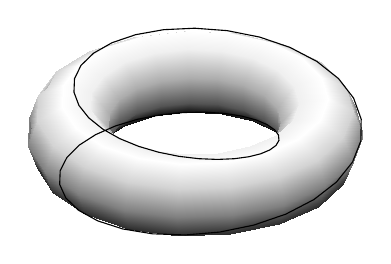
\begin{tikzpicture}
        \begin{axis}[
            hide axis,
            axis equal image,
            shader=interp,
            samples=20,
            samples y=10,
            xmin=-5, xmax=5,
            ymin=-5, ymax=5,
            zmin=-2, zmax=2,
            colormap/blackwhite,
            view={20}{30},
        ]

        \addplot3[
            surf,
            domain=0:360,
            y domain=0:360,
            z buffer=sort
        ]
        (
            {(3 + cos(y))*cos(x)},
            {(3 + cos(y))*sin(x)},
            {sin(y)}
        );

        \addplot3[
            samples=60,
            domain=0:360,
        ]
        (
            {(3 + cos(x))*cos(2*x)},
            {(3 + cos(x))*sin(2*x)},
            {sin(x)}
        );

        \end{axis}
    \end{tikzpicture}

    and here is a drawing of the lift to $\RR^2$

    \begin{tikzpicture}
        \begin{axis}[
            axis lines=middle,
            xmin=-5, xmax=5,
            ymin=-5, ymax=5,
        ]

            \addplot[
                domain=-10:10
            ]
                {2*x};

        \end{axis}
    \end{tikzpicture}

    \item[8.] Suppose $p: E \rightarrow B$ is a covering map, with $E$ path connected and $B$ simply connected.
    Then for any $b \in B$, $\pi_1(B,b) = \{e\}$ the trivial group. Theorem 54.4 says that the 
    map $\phi: \pi_1(B,b) \rightarrow p^{-1}(b)$ is surjective, so we must have that $p^{-1}(b)$ contains
    one element for all $b \in B$. Then $p$ must be injective. Moreover, since $p$ is a covering map, 
    we know that it is continuous, open, and surjective. Then $p$ is a homeomorphism.

\end{enumerate}

\end{document}